%\section{Gas Cerenkov}

\subsection{Gas Cerenkov Detectors}

 On both HRS, Gas Cherenkov Detectors (GC) are the main tools to identify pions and electrons. Although pions by design do not directly produce Cherenkov light in the GC, electrons knocked out by pions from gas atoms can fire the detectors and produce signals in the ADC spectra. However, we can identify those signals by considering that their are much weaker than ones produced by scattered electrons. Light radiated by an electron is collected by ten PMTs attached to ten mirrors inside each detector. After ADC channels of each PMT well aligned to represent the same energy scale, the sum of ten ADC signals should be proportional to energy carried by the electron, hence cutting on low values of ADC sum should remove most of pions. We aligned the single photon-electron peak (SPE) of each ADC at around 100 channels by timing a gain factor:
\begin{equation}
 C_{i} = \frac{100}{M_{i}^{SPE}-M_{i}^{pedestal}}
\end{equation}

\begin{figure}[h!]
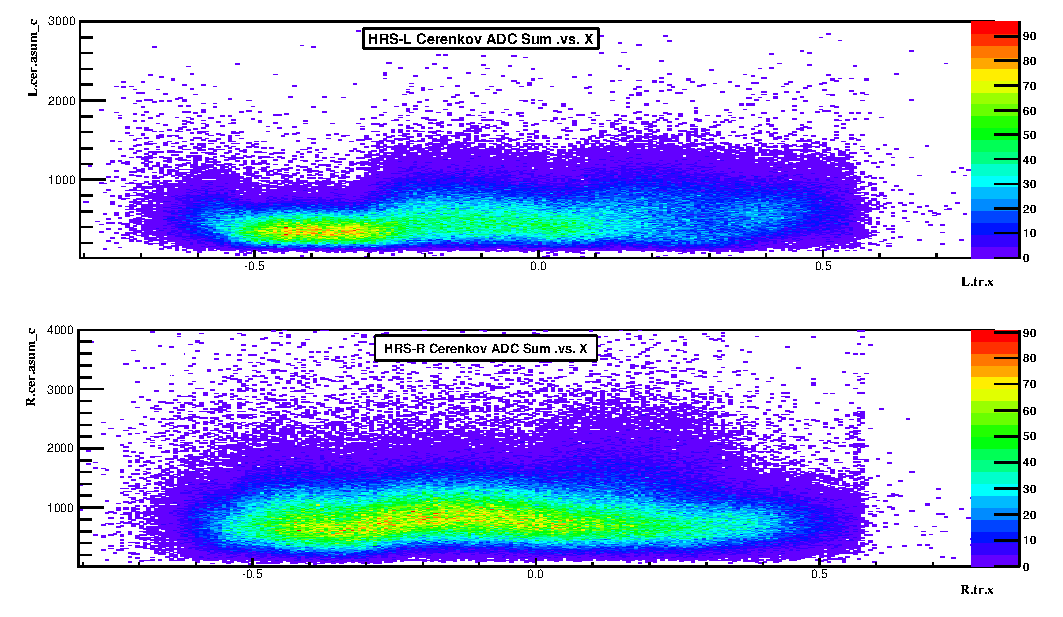
\includegraphics[width=0.48\linewidth]{figures/cer/Cerenkov_ADC_Align_Before.eps}
\hfill
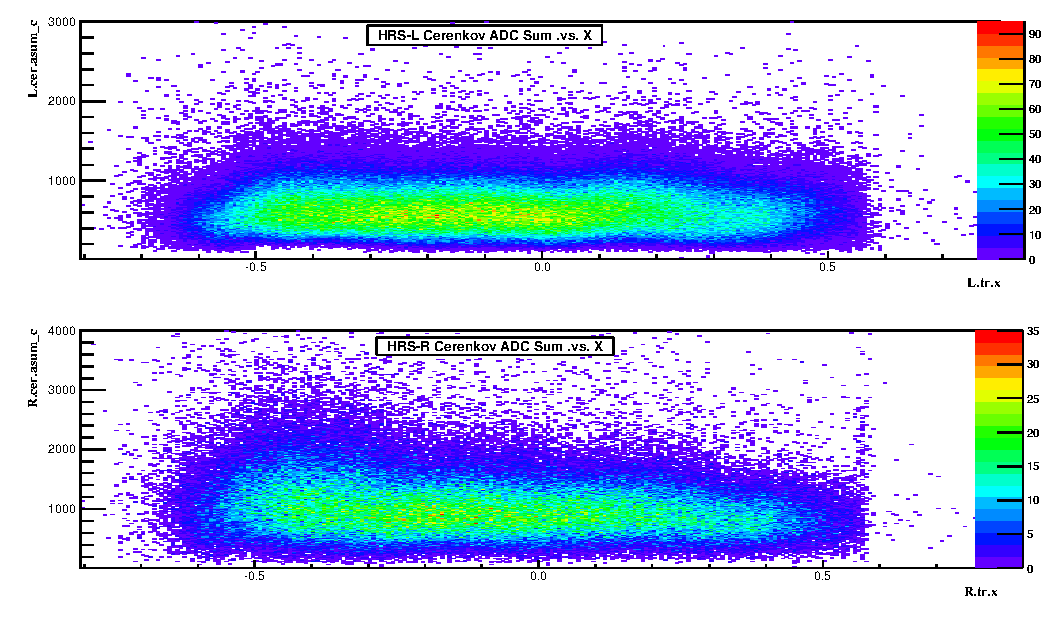
\includegraphics[width=0.48\linewidth]{figures/cer/Cerenkov_ADC_Align_After.eps}
\caption{\footnotesize{ADC Sum vs Tracking X before and after GC calibration}}
\label{gc_x}
\end{figure}

 where $M_{i}^{SPE}$ and $M_{i}^{pedestal}$ are the mean values of SPE peak and pedestal peak for the $ith$ PMT, fitted by a Gaussian function. The SPE peaks are not significant in our main production triggers ($T1\&T3$), so we perform the calibration with events from T6 and T7 since they do not include GC in the triggers. The improvement of calibration can be demonstrated by Fig~\ref{gc_x}, where the smooth distribution along X axis shows that each ADC is aligned properly. Single photon peaks are aligned to 100 channels after the calibration (Fig~\ref{cer_spe}). The calibration stability was also checked for each momentum setting (Fig~\ref{gc_stability}).

\parbox[t]{0.4\textwidth}{
 \includegraphics[width=\linewidth]{figures/cer/Cer_SPE.eps}
 \captionof{figure}{\footnotesize{GC SPE}}
 \label{cer_spe}
}
\hfill
\parbox[t]{0.5\textwidth}{
 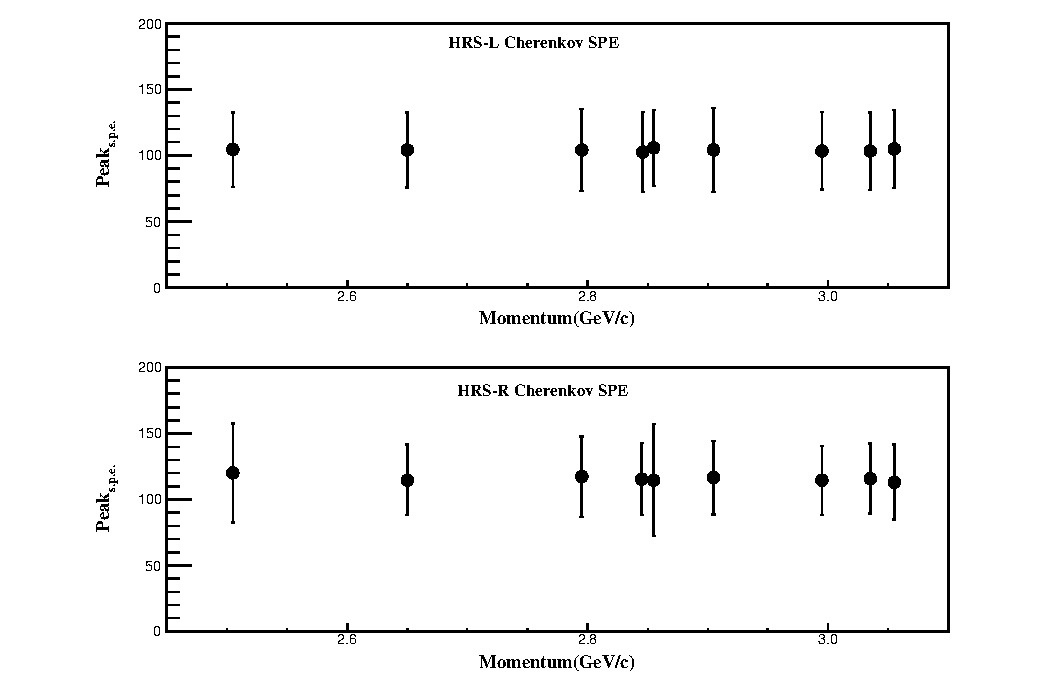
\includegraphics[width=\linewidth]{figures/cer/Cer_SPE_Err.eps}
\captionof{figure}{\footnotesize{Cerenkov SPE vs momentum}}
 \label{gc_stability}
}
